\section{Versuchsaufbau und Durchführung}
\label{sec:Durchführung}
Der Versuchsaufbau wird schematisch in der Abbildung \ref{fig:versuchsaufbau} dargestellt. Da die $\alpha$-Teilchen eine geringe Reichweite($\SI{10}{\centi\meter}$) in Luft haben, wird der Versuch in Vakuum durchgeführt, um die Wechselwirkung mit den Stoßpartnern(Luftmolekülen), an die die $\alpha$-Teilchen ihre kinetische Energie sukzessive abgeben, zu verhindern. Als Quelle dient ein $^{241}$Am-Präparat, das mit einer Halbwertszeit von $420$ Jahren zu Neptunium zerfällt. Die $\alpha$-Teilchen haben eine Energie von $\SI{5,486}{\mega\electronvolt}$.

\begin{figure}[h!]
	\centering
	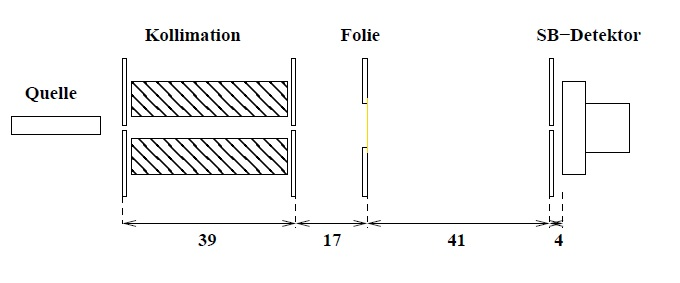
\includegraphics[width=0.9\linewidth]{../Versuchsaufbau}
	\caption{Zu sehen ist der schematische Aufbau des Versuches. Der Abstand zwischen den einzelnen Bauteilen der Messapparatur werden in Millimeter angegeben \cite[2]{anleitungV16}.}
	\label{fig:versuchsaufbau}
\end{figure}

Die Strahlen aus der Quelle werden mithilfe von zwei $\SI{2}{\milli\meter}$ Schlitzblenden kollimiert und werden durch die Blenden gebündelt. Der Strahl trifft anschließend senkrecht auf die Goldfolie, wo dann die Wechselwirkung mit Materie stattfindet. Die gestreuten $\alpha$-Teilchen werden in Abhängigkeit des Streuwinkels von einem Halbleiter-Detektor, also einem Surface-Barrier-Detektor detektiert. Bei diesem Detektor handelt es sich um eine in Sperrrichtung betriebene Diode, in der die einfallenden $\alpha$-Teilchen Elektronen-Loch-Paare erzeugen, die zur Elektrode beschleunigt werden. Der aufgenommene Impuls wird durch einen Multiplier verstärkt und ist proportional zur Energie des Teilchens. Außerdem sind ein Oszilloskop für die Energieverlustmessung und ein Zähler für die Streuquerschnittmessung vorhanden.

Zuerst wird die Streukammer mit einer Vakuumpumpe evakuiert. Die Sperrspannung des Surface-Barrier-Detektors wird auf $\SI{12}{\volt}$ eingestellt. Der Detektor wird justiert, um einen geraden Durchtritt  der $\alpha$-Teilchen zu gewährleisten. Anschließend wird eine Energieverlustmessung der Foliendicke durchgeführt. Dazu wird die Pulshöhe der Detektorpulse in Abhängigkeit von verschiedenen Kammerdrücken gemessen. Dieser Messvorgang wird zunächst mit und anschließend ohne eingesetzter Folie durchgeführt. Mithilfe von einem Feindrosselventil wird der Kammerdruck langsam erhöht. Zur Ermittlung der mittleren Pulshöhe wird das Oszilloskop in das Programm "Nachleuchten" gestellt, an dem dann die Pulshöhen abgelesen werden können. Im weiteren Verlauf des Versuches soll der differentielle Streuquerschnitt für eine $\SI{2}{\micro\meter}$ dünne Goldfolie untersucht werden. Hierfür wird die Zählrate in Abhängigkeit des Streuwinkels gemessen. Für diese Messung werden verschiedene Winkel eingestellt. Da der der $\alpha$-Zerfall poissonverteilt ist, wird versucht den Fehler möglichst klein zu halten. Der statistische Fehler dieser Messung für die Zählrate beträgt $\sqrt{I}$. Für die Messung der Mehrfachstreuung wird der Streuquerschnitt mithilfe von einer anderen Goldfolie mit einer Dicke von $\SI{4}{\micro\meter}$ bei einem festen Winkel von $15 ^\circ$ gemessen.

